\documentclass[border=8pt]{standalone}
\usepackage[T1]{fontenc}\usepackage{helvet}\renewcommand{\familydefault}{\sfdefault}
\usepackage{tikz}\usetikzlibrary{arrows.meta, positioning, calc, backgrounds}
\definecolor{ink}{HTML}{1a1916}
\definecolor{inktwo}{HTML}{3a3a35}
\definecolor{inkthree}{HTML}{6a6862}
\definecolor{rule}{HTML}{b8b09a}
\definecolor{amber}{HTML}{a8730a}
\definecolor{red}{HTML}{c8261a}
\definecolor{paper}{HTML}{f0eee5}
\definecolor{slab}{HTML}{d8d4c6}
\tikzset{
  >={Stealth[length=2.2mm]},
  wire/.style={line width=0.8pt, ink},
  modwire/.style={line width=0.6pt, dashed, ink},
  tastewire/.style={line width=0.6pt, dashed, amber},
  gatewire/.style={line width=0.6pt, dotted, ink},
  block/.style={rectangle, draw=ink, line width=0.9pt, fill=slab, minimum width=3.0cm, minimum height=1.9cm, inner sep=0pt},
  perf/.style={rectangle, draw=ink, line width=0.7pt, minimum width=3.0cm, minimum height=0.7cm, inner sep=2pt, font=\footnotesize, text=ink},
  title/.style={font=\scriptsize\bfseries, text=ink, anchor=north, inner sep=2pt},
  jack/.style={circle, draw=ink, fill=paper, line width=0.5pt, minimum size=3.2pt, inner sep=0pt},
  plabel/.style={font=\tiny, text=inktwo, anchor=west, inner sep=1pt},
  olabel/.style={font=\tiny, text=inktwo, anchor=east, inner sep=1pt},
  settings/.style={font=\scriptsize, text=ink, align=left, anchor=north west, inner sep=1pt, text width=2.9cm},
}
\begin{document}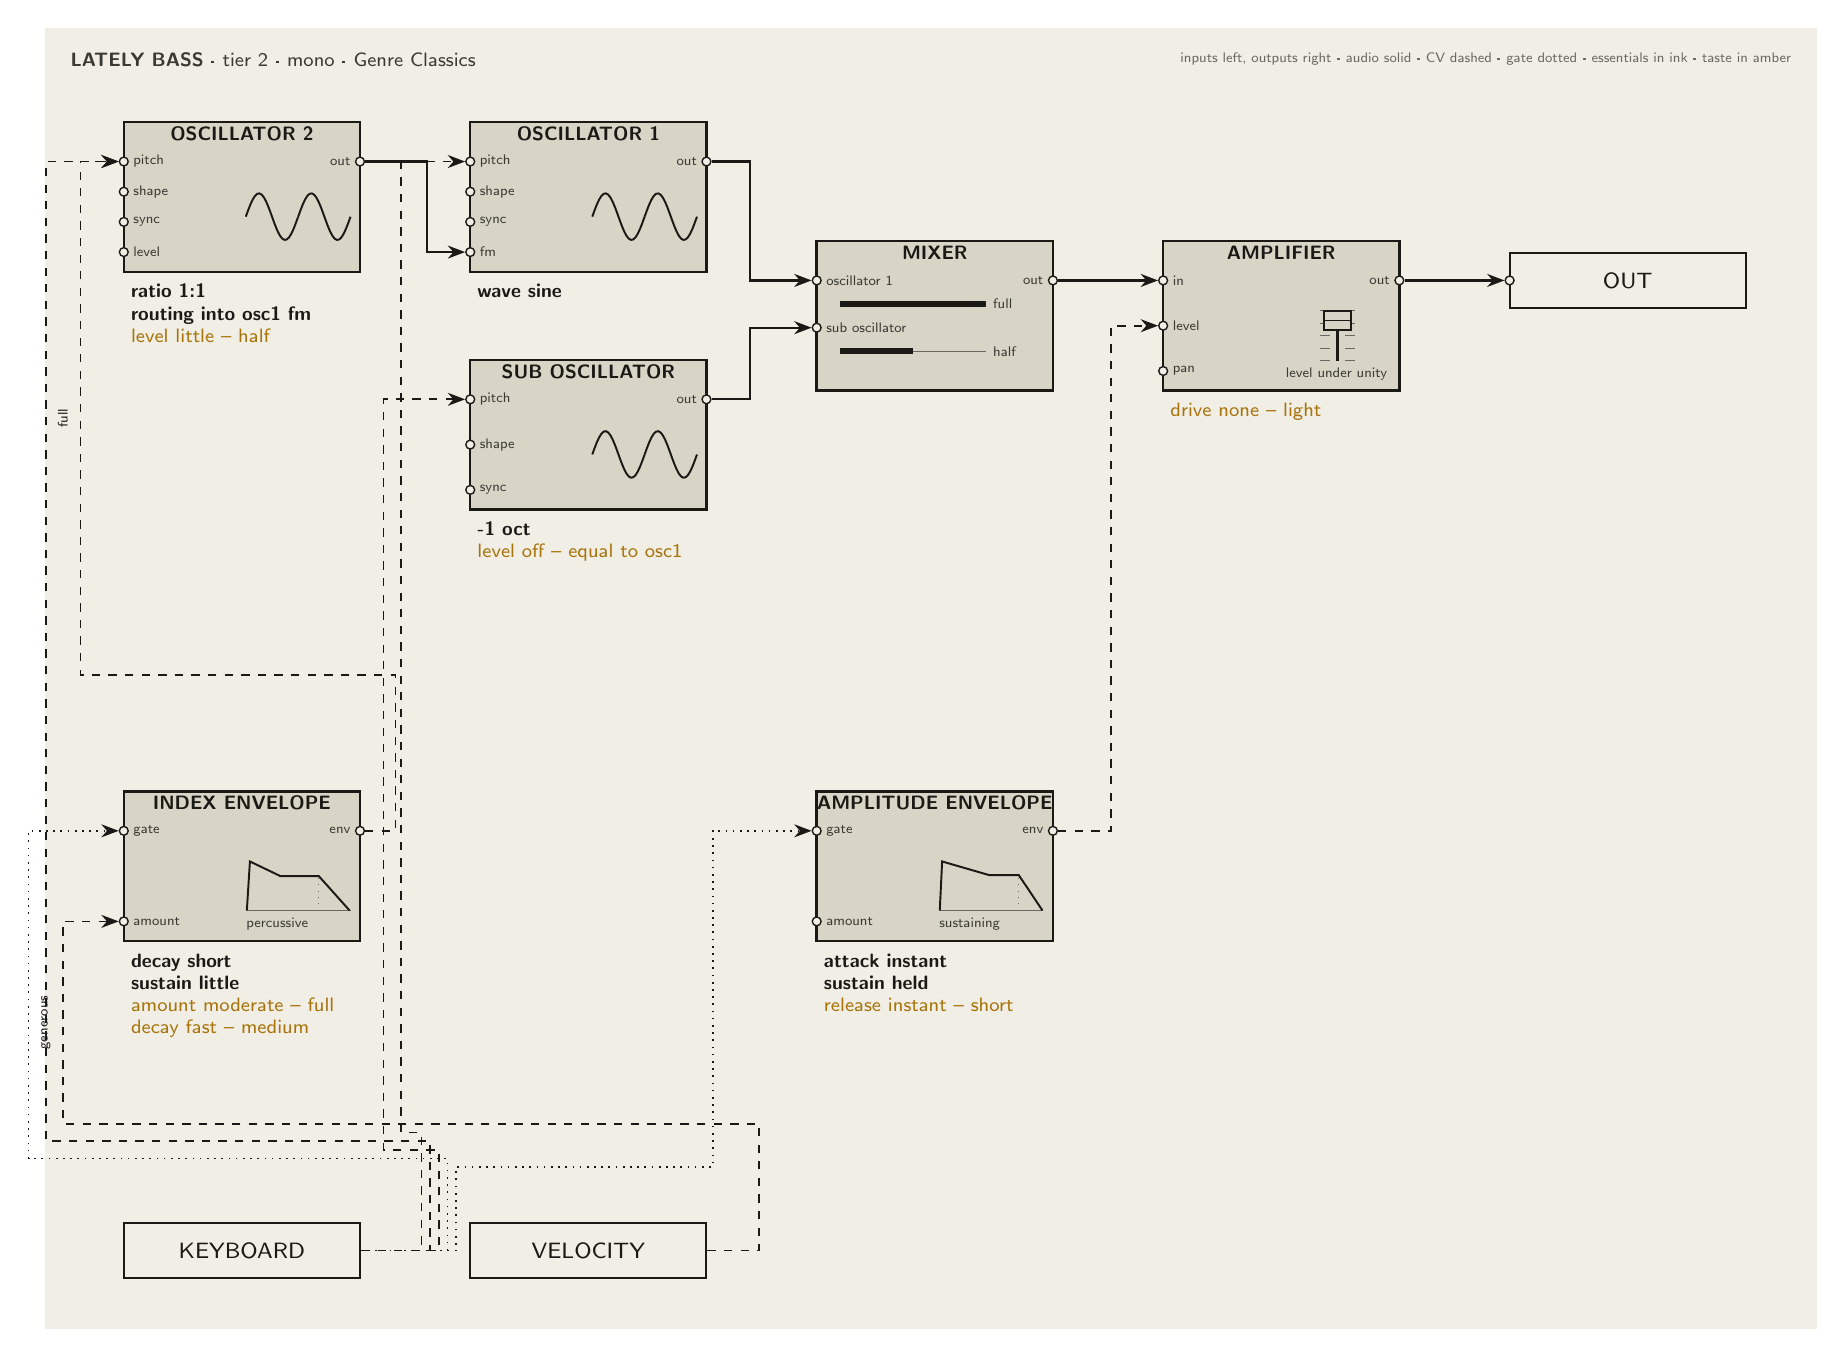
\begin{tikzpicture}
\begin{scope}[on background layer]\fill[paper] (-2.5,-12.870000000000001) rectangle (20.0,3.66);\end{scope}
\node[block, minimum height=1.9cm] (osc1) at (4.4,1.51) {};
\node[title] at (osc1.north) {OSCILLATOR 1};
\node[jack] (osc1-pitch) at (2.9000000000000004,1.96) {};
\node[plabel] at (2.9800000000000004,1.96) {pitch};
\node[jack] (osc1-shape) at (2.9000000000000004,1.5766666666666667) {};
\node[plabel] at (2.9800000000000004,1.5766666666666667) {shape};
\node[jack] (osc1-sync) at (2.9000000000000004,1.1933333333333334) {};
\node[plabel] at (2.9800000000000004,1.1933333333333334) {sync};
\node[jack] (osc1-fm) at (2.9000000000000004,0.81) {};
\node[plabel] at (2.9800000000000004,0.81) {fm};
\node[jack] (osc1-out) at (5.9,1.96) {};
\node[olabel] at (5.82,1.96) {out};
\begin{scope}
\draw[ink, line width=0.7pt] plot[domain=0.000:0.500, samples=24, variable=\u] ({4.450+\u*1.330},{0.890+(0.740)*(0.5+0.4*sin(360*(\u*2))+0.0)});
\draw[ink, line width=0.7pt] plot[domain=0.500:1.000, samples=24, variable=\u] ({4.450+\u*1.330},{0.890+(0.740)*(0.5+0.4*sin(360*(\u*2))+0.0)});
\end{scope}
\node[settings] at (2.95,0.44000000000000006) {\textbf{wave sine}};
\node[block, minimum height=1.9cm] (sub) at (4.4,-1.51) {};
\node[title] at (sub.north) {SUB OSCILLATOR};
\node[jack] (sub-pitch) at (2.9000000000000004,-1.06) {};
\node[plabel] at (2.9800000000000004,-1.06) {pitch};
\node[jack] (sub-shape) at (2.9000000000000004,-1.635) {};
\node[plabel] at (2.9800000000000004,-1.635) {shape};
\node[jack] (sub-sync) at (2.9000000000000004,-2.21) {};
\node[plabel] at (2.9800000000000004,-2.21) {sync};
\node[jack] (sub-out) at (5.9,-1.06) {};
\node[olabel] at (5.82,-1.06) {out};
\begin{scope}
\draw[ink, line width=0.7pt] plot[domain=0.000:0.500, samples=24, variable=\u] ({4.450+\u*1.330},{-2.130+(0.740)*(0.5+0.4*sin(360*(\u*2))+0.0)});
\draw[ink, line width=0.7pt] plot[domain=0.500:1.000, samples=24, variable=\u] ({4.450+\u*1.330},{-2.130+(0.740)*(0.5+0.4*sin(360*(\u*2))+0.0)});
\end{scope}
\node[settings] at (2.95,-2.58) {\textbf{-1 oct} \\ \textcolor{amber}{level off -- equal to osc1}};
\node[block, minimum height=1.9cm] (osc2) at (0.0,1.51) {};
\node[title] at (osc2.north) {OSCILLATOR 2};
\node[jack] (osc2-pitch) at (-1.5,1.96) {};
\node[plabel] at (-1.42,1.96) {pitch};
\node[jack] (osc2-shape) at (-1.5,1.5766666666666667) {};
\node[plabel] at (-1.42,1.5766666666666667) {shape};
\node[jack] (osc2-sync) at (-1.5,1.1933333333333334) {};
\node[plabel] at (-1.42,1.1933333333333334) {sync};
\node[jack] (osc2-level) at (-1.5,0.81) {};
\node[plabel] at (-1.42,0.81) {level};
\node[jack] (osc2-out) at (1.5,1.96) {};
\node[olabel] at (1.42,1.96) {out};
\begin{scope}
\draw[ink, line width=0.7pt] plot[domain=0.000:0.500, samples=24, variable=\u] ({0.050+\u*1.330},{0.890+(0.740)*(0.5+0.4*sin(360*(\u*2))+0.0)});
\draw[ink, line width=0.7pt] plot[domain=0.500:1.000, samples=24, variable=\u] ({0.050+\u*1.330},{0.890+(0.740)*(0.5+0.4*sin(360*(\u*2))+0.0)});
\end{scope}
\node[settings] at (-1.45,0.44000000000000006) {\textbf{ratio 1:1} \\ \textbf{routing into osc1 fm} \\ \textcolor{amber}{level little -- half}};
\node[block, minimum height=1.9cm] (mix) at (8.8,0.0) {};
\node[title] at (mix.north) {MIXER};
\node[jack] (mix-osc1) at (7.300000000000001,0.44999999999999996) {};
\node[plabel] at (7.380000000000001,0.44999999999999996) {oscillator 1};
\draw[inkthree, line width=0.3pt] (7.600,0.150) -- (9.450,0.150);
\draw[ink, line width=2.2pt] (7.600,0.150) -- (9.450,0.150);
\node[font=\tiny, text=inktwo, anchor=west, inner sep=1pt] at (9.500,0.150) {full};
\node[jack] (mix-sub) at (7.300000000000001,-0.15000000000000002) {};
\node[plabel] at (7.380000000000001,-0.15000000000000002) {sub oscillator};
\draw[inkthree, line width=0.3pt] (7.600,-0.450) -- (9.450,-0.450);
\draw[ink, line width=2.2pt] (7.600,-0.450) -- (8.525,-0.450);
\node[font=\tiny, text=inktwo, anchor=west, inner sep=1pt] at (9.500,-0.450) {half};
\node[jack] (mix-out) at (10.3,0.44999999999999996) {};
\node[olabel] at (10.22,0.44999999999999996) {out};
\node[block, minimum height=1.9cm] (amp) at (13.200000000000001,0.0) {};
\node[title] at (amp.north) {AMPLIFIER};
\node[jack] (amp-in) at (11.700000000000001,0.44999999999999996) {};
\node[plabel] at (11.780000000000001,0.44999999999999996) {in};
\node[jack] (amp-level) at (11.700000000000001,-0.125) {};
\node[plabel] at (11.780000000000001,-0.125) {level};
\node[jack] (amp-pan) at (11.700000000000001,-0.7) {};
\node[plabel] at (11.780000000000001,-0.7) {pan};
\node[jack] (amp-out) at (14.700000000000001,0.44999999999999996) {};
\node[olabel] at (14.620000000000001,0.44999999999999996) {out};
\begin{scope}
\draw[ink, line width=1.2pt] (13.915,-0.570) -- (13.915,0.070);
\draw[inkthree, line width=0.3pt] (13.695,-0.570) -- (13.815,-0.570) (14.015,-0.570) -- (14.135,-0.570);
\draw[inkthree, line width=0.3pt] (13.695,-0.410) -- (13.815,-0.410) (14.015,-0.410) -- (14.135,-0.410);
\draw[inkthree, line width=0.3pt] (13.695,-0.250) -- (13.815,-0.250) (14.015,-0.250) -- (14.135,-0.250);
\draw[inkthree, line width=0.3pt] (13.695,-0.090) -- (13.815,-0.090) (14.015,-0.090) -- (14.135,-0.090);
\draw[inkthree, line width=0.3pt] (13.695,0.070) -- (13.815,0.070) (14.015,0.070) -- (14.135,0.070);
\fill[slab, draw=ink, line width=0.6pt] (13.745,-0.178) rectangle (14.085,0.062);
\draw[ink, line width=0.5pt] (13.745,-0.058) -- (14.085,-0.058);
\node[font=\tiny, text=inktwo, anchor=north west, inner sep=0pt] at (13.250,-0.650) {level under unity};
\end{scope}
\node[settings] at (11.750000000000002,-1.0699999999999998) {\textcolor{amber}{drive none -- light}};
\node[block, minimum height=1.9cm] (menv) at (0.0,-6.99) {};
\node[title] at (menv.north) {INDEX ENVELOPE};
\node[jack] (menv-gate) at (-1.5,-6.54) {};
\node[plabel] at (-1.42,-6.54) {gate};
\node[jack] (menv-amount) at (-1.5,-7.6899999999999995) {};
\node[plabel] at (-1.42,-7.6899999999999995) {amount};
\node[jack] (menv-out) at (1.5,-6.54) {};
\node[olabel] at (1.42,-6.54) {env};
\begin{scope}
\draw[inkthree, line width=0.3pt] (0.050,-7.551) -- (1.380,-7.551);
\draw[ink, line width=0.7pt] (0.063,-7.551) -- (0.102,-6.929) -- (0.491,-7.116) -- (0.978,-7.116) -- (1.367,-7.551);
\draw[inkthree, line width=0.3pt, dotted] (0.978,-7.551) -- (0.978,-7.116);
\node[font=\tiny, text=inktwo, anchor=north west, inner sep=0pt] at (0.050,-7.640) {percussive};
\end{scope}
\node[settings] at (-1.45,-8.06) {\textbf{decay short} \\ \textbf{sustain little} \\ \textcolor{amber}{amount moderate -- full} \\ \textcolor{amber}{decay fast -- medium}};
\node[block, minimum height=1.9cm] (aenv) at (8.8,-6.99) {};
\node[title] at (aenv.north) {AMPLITUDE ENVELOPE};
\node[jack] (aenv-gate) at (7.300000000000001,-6.54) {};
\node[plabel] at (7.380000000000001,-6.54) {gate};
\node[jack] (aenv-amount) at (7.300000000000001,-7.6899999999999995) {};
\node[plabel] at (7.380000000000001,-7.6899999999999995) {amount};
\node[jack] (aenv-out) at (10.3,-6.54) {};
\node[olabel] at (10.22,-6.54) {env};
\begin{scope}
\draw[inkthree, line width=0.3pt] (8.850,-7.551) -- (10.180,-7.551);
\draw[ink, line width=0.7pt] (8.863,-7.551) -- (8.893,-6.929) -- (9.493,-7.103) -- (9.867,-7.103) -- (10.167,-7.551);
\draw[inkthree, line width=0.3pt, dotted] (9.867,-7.551) -- (9.867,-7.103);
\node[font=\tiny, text=inktwo, anchor=north west, inner sep=0pt] at (8.850,-7.640) {sustaining};
\end{scope}
\node[settings] at (7.3500000000000005,-8.06) {\textbf{attack instant} \\ \textbf{sustain held} \\ \textcolor{amber}{release instant -- short}};
\node[perf] (key) at (0.0,-11.870000000000001) {KEYBOARD};
\node[perf] (vel) at (4.4,-11.870000000000001) {VELOCITY};
\node[perf, fill=paper] (out) at (17.6,0.44999999999999996) {OUT}; \node[jack] (out-in) at (16.1,0.44999999999999996) {};
\draw[wire,->] (osc2-out) -- (2.3500000000000005,1.96) -- (2.3500000000000005,0.81) -- (osc1-fm);
\draw[wire,->] (osc1-out) -- (6.45,1.96) |- (mix-osc1);
\draw[wire,->] (sub-out) -- (6.45,-1.06) |- (mix-sub);
\draw[wire,->] (mix-out) -- (amp-in);
\draw[wire,->] (amp-out) -- (out-in);
\draw[modwire,->] (menv-out) -- (1.95,-6.54) -- (1.95,-4.5600000000000005) -- (-2.05,-4.5600000000000005) -- (-2.05,1.96) -- (osc2-pitch);
\node[font=\tiny, text=ink, anchor=south, inner sep=1pt, rotate=90] at (-2.17,-1.3000000000000003) {full};
\draw[modwire,->] (aenv-out) -- (11.040000000000001,-6.54) -- (11.040000000000001,-0.125) -- (amp-level);
\draw[modwire,->] (vel.east) -- (6.57,-11.870000000000001) -- (6.57,-10.260000000000002) -- (-2.27,-10.260000000000002) -- (-2.27,-7.6899999999999995) -- (menv-amount);
\node[font=\tiny, text=ink, anchor=south, inner sep=1pt, rotate=90] at (-2.39,-8.975000000000001) {generous};
\draw[modwire,->] (key.east) -- (2.28,-11.870000000000001) -- (2.28,-10.370000000000001) -- (2.0200000000000005,-10.370000000000001) -- (2.0200000000000005,1.96) -- (osc1-pitch);
\draw[modwire,->] (key.east) -- (2.39,-11.870000000000001) -- (2.39,-10.48) -- (-2.4899999999999998,-10.48) -- (-2.4899999999999998,1.96) -- (osc2-pitch);
\draw[modwire,->] (key.east) -- (2.5,-11.870000000000001) -- (2.5,-10.590000000000002) -- (1.8000000000000005,-10.590000000000002) -- (1.8000000000000005,-1.06) -- (sub-pitch);
\draw[gatewire,->] (key.east) -- (2.61,-11.870000000000001) -- (2.61,-10.700000000000001) -- (-2.71,-10.700000000000001) -- (-2.71,-6.54) -- (menv-gate);
\draw[gatewire,->] (key.east) -- (2.7199999999999998,-11.870000000000001) -- (2.7199999999999998,-10.81) -- (5.98,-10.81) -- (5.98,-6.54) -- (aenv-gate);
\node[anchor=north west, font=\scriptsize, text=inktwo] at (-2.3,3.46) {\textbf{LATELY BASS} · tier 2 · mono · Genre Classics};
\node[anchor=north east, font=\tiny, text=inkthree] at (19.8,3.46) {inputs left, outputs right · audio solid · CV dashed · gate dotted · essentials in ink · taste in amber};
\end{tikzpicture}\end{document}
